%! suppress = TooLargeSection
%! suppress = SentenceEndWithCapital
%! suppress = TooLargeSection
% Preamble
\documentclass[11pt]{PyRollDocs}
\usepackage{textcomp}
\usepackage{csquotes}
\usepackage{wasysym}

\addbibresource{refs.bib}
% Document
\begin{document}

    \title{Elastic work roll deformation PyRoll Plugin}
    \author{Christoph Renzing}
    \date{\today}

    \maketitle

    This plugin provides the so-called matrix method to calculate the elastic deformation of the work roll.
    Besides the deflection, also the corresponding inclination angle as well as the shear force and bending moment are calculated.


    \section{Model approach}\label{sec:model-approach}

    The core idea is to consider the roll as a prismatic rod with varying diameter and discretize
    its length into $n$ disks with length $dz$, which are subjected to a constant linear load $q$ and have a locally constant $I$.
    Every disk has four state variables, which are the deflection $v$,
    the inclination $\alpha$, the bending moment $M_B$ and the shear force $F_Q$.
    These four variables unambiguously determine the deformation and stress state of a disc.
    The values of the state variables at entry and exit of each disk are denoted by the indizes $0$ and $1$ (see Figure~\ref{fig:exemplary-roll-and-disk}).

    \begin{figure}
        \centering
        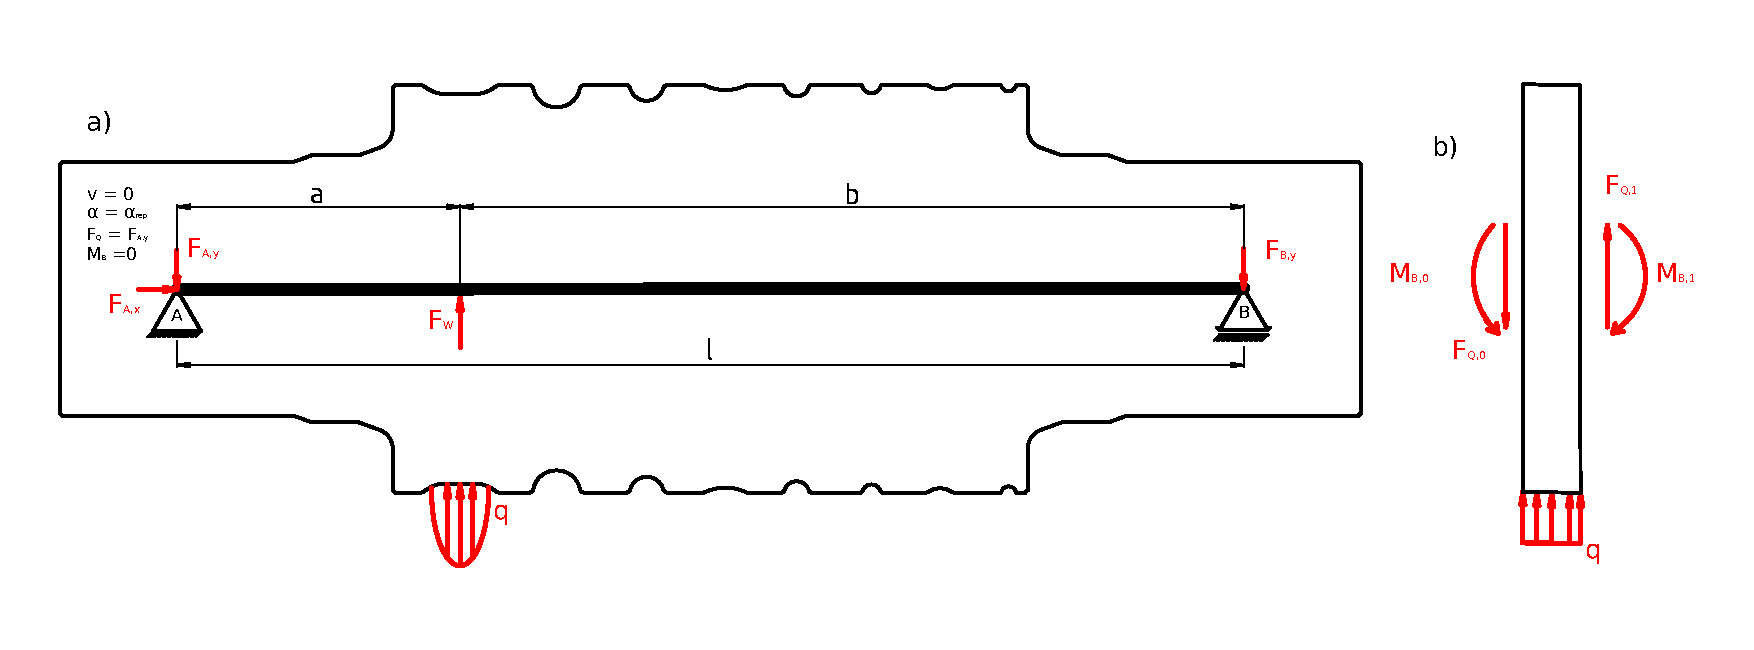
\includegraphics[width=\linewidth]{img/exemplary-roll}
        \caption{(a) Work roll for break down mill of the semi-continuous rolling plant at the institute of metal forming with exemplary load distribution and mechanical substitute system; (b) disk element used for discretization}
        \label{fig:exemplary-roll-and-disk}
    \end{figure}

    Solving the 4th order differential equation for the deflection (see equation~\eqref{eq:fourth-order-deflection}) of a disk between its boundaries,
    under consideration of the above assumptions, allows the equations to be expressed as matrix.
    The resulting matrix is called \emph{transition matrix} as it accomplishes the transition of the state variables in each disk.
    The entry state of the following disk can be calculated using the exit state of the previous disk through equation~\eqref{eq:matrix-method}.
    As \textcite{Becker_König_Guericke_Hinkfoth_1979} and \textcite{Kulbatschny_1954} stated,
    the bearings of a roll are designed to be free of bending moments and have a very high bending rigidity.
    \textcite{Göldner_Holzweißig_1989} suggests,
    that bearings can therefore be modeled using spring constants resulting in a special transfer matrix for bearings.
    Since it was not possible to measure the necessary constants for the respective plant, the spring constant and the
    torsion spring constant were assumed to be $\infty$ and $0$, respectively.
    Furthermore, the bearing of the roll was approximated to be located at the center of each roll joints.
    In order to better represent the load on the roll resulting from the process,
    it was assumed that the pressure distribution in the contact area between the rolled material and the roll is elliptical and has its maximum in the centre of the groove.
    The width of the ellipse is equal to the width in which the rolled stock experiences hindered spreading.
    This width was calculated according to the model of \textcite{Lendl_1948a}.
    A similar assumption was made by \textcite{Hitchcock_Trinks_1935} for elastic flattening of the roll, but in rolling direction.
    The assumptions can bee seen in \autoref{fig:exemplary-roll-and-disk}.

    \begin{equation}
        E I v '''' = q
        \label{eq:fourth-order-deflection}
    \end{equation}

    \begin{equation}
        \begin{pmatrix}
            v  \\[2pt]
            \alpha     \\[2pt]
            M_B \\[2pt]
            F_Q    \\[2pt]
            1              \\[2pt]
        \end{pmatrix}_{1}
        =
        \begin{pmatrix}
            1 & dz & \frac{dz^2}{2 E I} & \frac{dz^3}{6 E I} & q \frac{dz^4}{24 E I} \\[2pt]
            0 & 1  & \frac{dz}{E I}     & \frac{dz^2}{2 E I} & q \frac{dz^3}{6 E I}  \\[2pt]
            0 & 0  & 1                  & dz                 & q \frac{dz^2}{2}                                      \\[2pt]
            0 & 0  & 0                  & 1                  & q dz                                                  \\[2pt]
            0 & 0  & 0                  & 0                  & 1                                                                           \\[2pt]
        \end{pmatrix}
        \begin{pmatrix}
            v  \\[2pt]
            \alpha     \\[2pt]
            M_B \\[2pt]
            F_Q   \\[2pt]
            1              \\[2pt]
        \end{pmatrix}_{0}
        \label{eq:matrix-method}
    \end{equation}

    For performing the calculation, the components of the vector in point A must be known.
    Deflection $v(A)$ and moment $M_B(A)$ are equal zero due to the assumptions.
    The shear force $F_Q(A)$ and inclination $\alpha(A)$ are unequal zero and must be determined numerically,
    so that the deflection $v(\PointB)$ and moment $M_B(\PointB)$ are zero in point B.

    \begin{equation}
        \begin{pmatrix}
            v  \\[2pt]
            \alpha     \\[2pt]
            M_B \\[2pt]
            F_Q   \\[2pt]
            1              \\[2pt]
        \end{pmatrix}_{A}
        =
        \begin{pmatrix}
            0  \\[2pt]
            \alpha(A)     \\[2pt]
            0 \\[2pt]
            F_Q(A)   \\[2pt]
            1              \\[2pt]
        \end{pmatrix}
        \label{eq:initial-vector}
    \end{equation}

    To estimate initial values for the numerical solution, a substitute system is used, namely the bending of a constant cross-section rod by a point force, as shown in \autoref{fig:exemplary-roll-and-disk}.
    The force balance on this system leads to the expressions in \autoref{eq:initial-values}.

    \begin{subequations}
        \begin{gather}
            F_Q(A) = -\Force_{A, \mathrm{y}} = -F_W \left( 1 - \frac{a}{l} \right)
            \label{eq:bearing-force}\\
            \alpha(A) = \frac{F_W a b \left( l + b \right)}{6 E bar{I} l}
            \label{eq:inclination}
        \end{gather}
        \label{eq:initial-values}
    \end{subequations}

    Using the initial solution, the final solution is computed using the HYBRD algorithm by \textcite{Powell} provided in Scipy~\cite{Virtanen_Gommers_Oliphant_Haberland_Reddy_Cournapeau_Burovski_Peterson_Weckesser_Bright_2020}.


    \section{Usage instructions}\label{sec:usage-instructions}

    The plugin can be loaded under the name \texttt{pyroll\_work\_roll\_elastic\_deformation}.
    Besides the hooks \lstinline{youngs_modulus}, the implemented \lstinline{body} hook is the entry point for the calculation.
    The calculation is done, using the classes \listinline{DiskElement}, \listinline{RollBody} and \listinline{MatrixMethod}.
    Several additional hooks on \lstinline{RollPass.Roll} are defined, which are used for calculation, as listed in \autoref{tab:hookspecs}.

    \begin{table}
        \centering
        \caption{Hooks specified by this plugin.}
        \label{tab:hookspecs}
        \begin{tabular}{ll}
            \toprule
            Hook name                        & Meaning                                                       \\
            \midrule
            \texttt{matrix\_method\_results} & Results of the matrix method as an array of arrays            \\
            \texttt{disk\_elements}          & Array of disk elements used for discretization of the grooves \\
            \texttt{deflection}              & Array of the deflection                                       \\
            \texttt{inclination}             & Array of the inclination                                      \\
            \texttt{bending\_moment}         & Array of the bending moment                                   \\
            \texttt{shear\_force}            & Array of the shear force                                      \\


            \bottomrule
        \end{tabular}
    \end{table}

    \printbibliography


\end{document}